\documentclass[12pt, oneside, a4paper]{scrreprt}

\usepackage[manualmark,headsepline,footsepline]{scrlayer-scrpage}

\usepackage[german]{babel}
\usepackage[utf8]{inputenc}
\usepackage{graphicx} %Grafik aktivieren
\usepackage{float}
\usepackage[final]{pdfpages}
\usepackage{hyperref}
\usepackage{pdfcomment}

\usepackage{siunitx}  
\sisetup{locale = DE,separate-uncertainty}  

\usepackage[backend=biber]{biblatex}
\addbibresource{refs.bib}


%% used for pgfplots, tikzpicture
\usepackage{pgfplots}
\pgfplotsset{compat=newest}

%% the following commands are needed for some matlab2tikz features
\usetikzlibrary{plotmarks}
\usetikzlibrary{arrows.meta}
\usetikzlibrary{datavisualization}
\usetikzlibrary{datavisualization.formats.functions}
\usepgfplotslibrary{patchplots}
\usepackage{array}
\usepackage{grffile} 
\usepackage{amsmath}

\usepackage{todonotes}

\usepackage{listings}

\pgfplotsset{plot coordinates/math parser=false}
\newlength\fwidth

%%%%%%%%%%%%%%%%%%%%%%%%%%%%%%%%%%%%%%%%%%%%%%%%%%%%%%%%%%%%%%%%%%%%%%%%%%%%%%%%%%%%%%%%%%%%%%%%%%%%%%%%%%%%%%%%%%%%%%%%

%Kapitel-Layout
\usepackage{lmodern} 
\usepackage{xcolor}
\colorlet{chapter}{black!75}
\addtokomafont{chapter}{\color{chapter}}
\makeatletter% siehe De-TeX-FAQ
\renewcommand*{\chapterformat}{%
    \begingroup% damit \unitlength-Änderung lokal bleibt 
    \setlength{\unitlength}{1mm}% 
    \begin{picture}(20,20)(0,5)% 
    \setlength{\fboxsep}{0pt}% 
    \put(20,20){\line(1,0){\dimexpr 
    \textwidth-20\unitlength\relax\@gobble}}% 
    \put(0,0){\makebox(15,20)[r]{% 
    \fontsize{18\unitlength}{28\unitlength}\selectfont\thechapter 
    \kern-.04em% Ziffer in der Zeichenzelle nach rechts schieben 
    }}% 
    \end{picture} % <-- Leerzeichen ist hier beabsichtigt! 
    \newline
    \endgroup
}

\setlength\parindent{0pt}

%%%%%%%%%%%%%%%%%%%%%%%%%%%%%%%%%%%%%%%%%%%%%%%%%%%%%%%%%%%%%%%%%%%%%%%%%%%%%%%%%%%%%%%%%%%%%%%%%%%%%%%%%%%%%%%%%%%%%%%%

% Kopf- und Fußzeilen, Seitenränder etc.
% Kopf- und Fußzeilen ------------------------------------------------------
\pagestyle{scrheadings}

% Kopf- und Fußzeile auch auf Kapitelanfangsseiten -------------------------
\renewcommand*{\chapterpagestyle}{scrheadings}

% Schriftform der Kopfzeile ------------------------------------------------
\renewcommand{\headfont}{%
\normalfont
}

% Kopfzeile ----------------------------------------------------------------
\ihead{Regelungstechnisches Praktikum (RTP)}
\chead{}
\ohead{
\includegraphics[width=0.3\textwidth]{figure/oth-regensburg-logo}}
%
\setlength{\headheight}{21mm} % Höhe der Kopfzeile
%\setheadsepline[text]{0.4pt} % Trennlinie unter Kopfzeile

% Fußzeile -----------------------------------------------------------------
\ifoot{Name 1 Name 2}
\cfoot{\today}
\ofoot{\pagemark}


% erzeugt ein wenig mehr Platz hinter einem Punkt --------------------------
\frenchspacing 

\clubpenalty = 10000
\widowpenalty = 10000 
\displaywidowpenalty = 10000


\newcommand{\mt}[1]{\textrm{#1}}



%%%%%%%%%%%%%%%%%%%%%%%%%%%%%%%%%%%%%%%%%%%%%%%%%%%%%%%%%%%%%%%%%%%%%%%%%%%%%%%%%%%%%%%%%%%%%%%%%%%%%%%%%%%%%%%%%%%%%%%%
%%%%%%%%%%%%%%%%%%%%%%%%%%%%%%%%%%%%%%%%%%%%%%%%%%%%%%%%%%%%%%%%%%%%%%%%%%%%%%%%%%%%%%%%%%%%%%%%%%%%%%%%%%%%%%%%%%%%%%%%
%%%%%%%%%%%%%%%%%%%%%%%%%%%%%%%%%%%%%%%%%%%%%%%%%%%%%%%%%%%%%%%%%%%%%%%%%%%%%%%%%%%%%%%%%%%%%%%%%%%%%%%%%%%%%%%%%%%%%%%%

\begin{document}
    \begin{titlepage}

        \begin{tabular}{l r} 
            
\includegraphics[width=0.4\textwidth]{figure/oth-regensburg-logo.jpg}
            &
        \end{tabular}

        \begin{minipage} [c] [8.5cm] [b] {\textwidth}
            \Huge{
                \begin{center}
                    \textbf{Praktikum Regelungstechnik (RTP)}\\[0.8cm]
                    \textbf{Versuch T3: RetBot system identification, part I} \\[1.5cm]
                    \par
                    {\large Versuch 3}\\[1cm]
                    {\large \today} \\[1cm]
                \end{center}
                }
        \end{minipage}

        \vspace{0.1cm}

        \begin{minipage} [c] [3.5cm] [b] {\textwidth}
            \begin{center}
                \vspace{0.3cm}
                Gruppe 38\\
                Marius Off\\
                Janis Graf\\
                \vspace{0.5cm}
                %\texttt{Dokument-Version: 02}\\
            \end{center}
        \end{minipage}

    \end{titlepage}

    \todo[inline]{go through whole document and check for consistency of formatting, notation, and style and SI package usage}
    \missingfigure{TASK: upload videos for two different duty-cycles moving alongside a folding rule!}
        

    \tableofcontents


    \chapter{Preperations}\label{chap:preperations}
    
        \section{(aV) Explanation of pulse width modulation control for a drive.}
            Pulse width modulation (PWM) is a technique used to control the power delivered to a load, such as a motor, by varying the width of the pulses in a pulse train. The duty cycle of the PWM signal determines the average voltage applied to the load, allowing for precise control of the motor's speed and torque.
            The important parameters of PWM include, the impulse width (the duration of the `on' time), the period (the total duration of one cycle), the break time (the duration of the `off' time), and the VCC span (the voltage level of the `on' and `off' states) as shown in Figure \ref{fig:PWM-parameters}.

            \begin{figure}
                \centering
                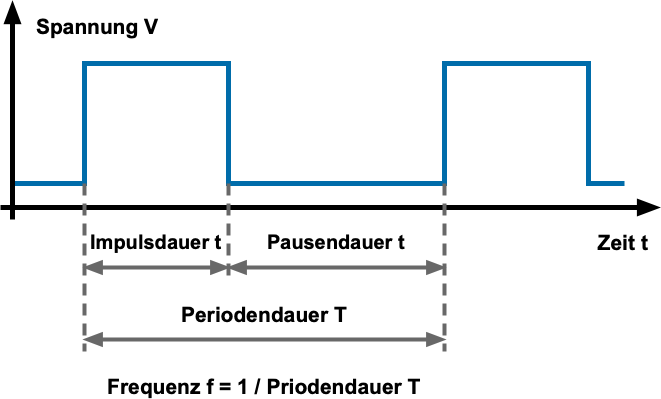
\includegraphics[width=0.8\textwidth, height=0.2\textheight, keepaspectratio]{figure/PWM-values.png}
                \caption{Illustration of PWM parameters\autocite{PWMPulsweitenmodulationPDM}}
                \label{fig:PWM-parameters}
            \end{figure}

            The duty cycles of the PWM signal can be adjusted to control the motor's behavior. See Figure \ref{fig:PWM-cycle} for example
            \begin{itemize}
                \item \SI{10}{\percent} duty cycle means the motor receives power for \SI{10}{\percent} of the time, and is off for the remaining 90%
                \item \SI{50}{\percent} duty cycle means the motor receives power for \SI{50}{\percent} of the time, and is off for the remaining 50%
                \item \SI{90}{\percent} duty cycle means the motor receives power for \SI{90}{\percent} of the time, and is off for the remaining 10%
            \end{itemize}

            \begin{figure}[ht]
                \centering
                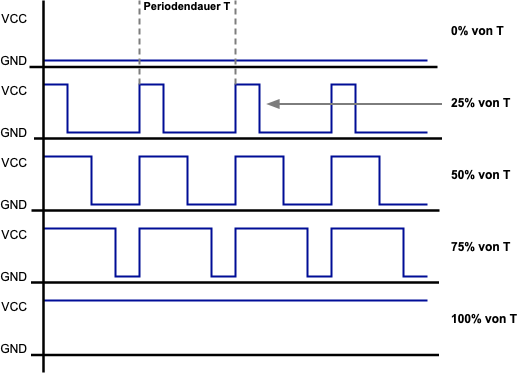
\includegraphics[width=0.8\textwidth, height=0.20\textheight, keepaspectratio]{figure/PWM-cycle.png}
                \caption{Illustration of PWM duty cycles\autocite{PWMPulsweitenmodulationPDM}}
                \label{fig:PWM-cycle}
            \end{figure}

        \cleardoublepage

        \section{(bV) Serial interface (RS232) and its key parameters}
            The RS232 interface is used for connecting devices together one sender and one receiver. Before USB it was one of the most common interfaces for connecting peripherals to computers. Both the sender and the receiver have to be configured with the same parameters for the communication to work. The key parameters are shown in figure \ref{fig:RS232} and include:

            \begin{itemize}
                \item Baud rate: The speed of data transmission, measured in bits per second (bps). Common baud rates include and range from 110, 9600, 19200, 38400, 57600, and 115200 bps.
                \item Data bits: The number of bits used to represent each character. Common settings are 7 or 8 data bits.
                \item Parity: A method of error checking. It can be set to none, even, odd, mark, or space.
                \item Stop bits: The number and configuration of stop bits used to signal the end of a data packet.
                \item Flow control: A method to control the flow of data between devices, which can be hardware (RTS/CTS) or software (XON/XOFF).
                \item Voltage levels: RS232 uses specific voltage levels for signaling, typically +3 to +15 volts for a logical '1' and -3 to -15 volts for a logical '0'.
            \end{itemize}

            \begin{figure}
                \centering
                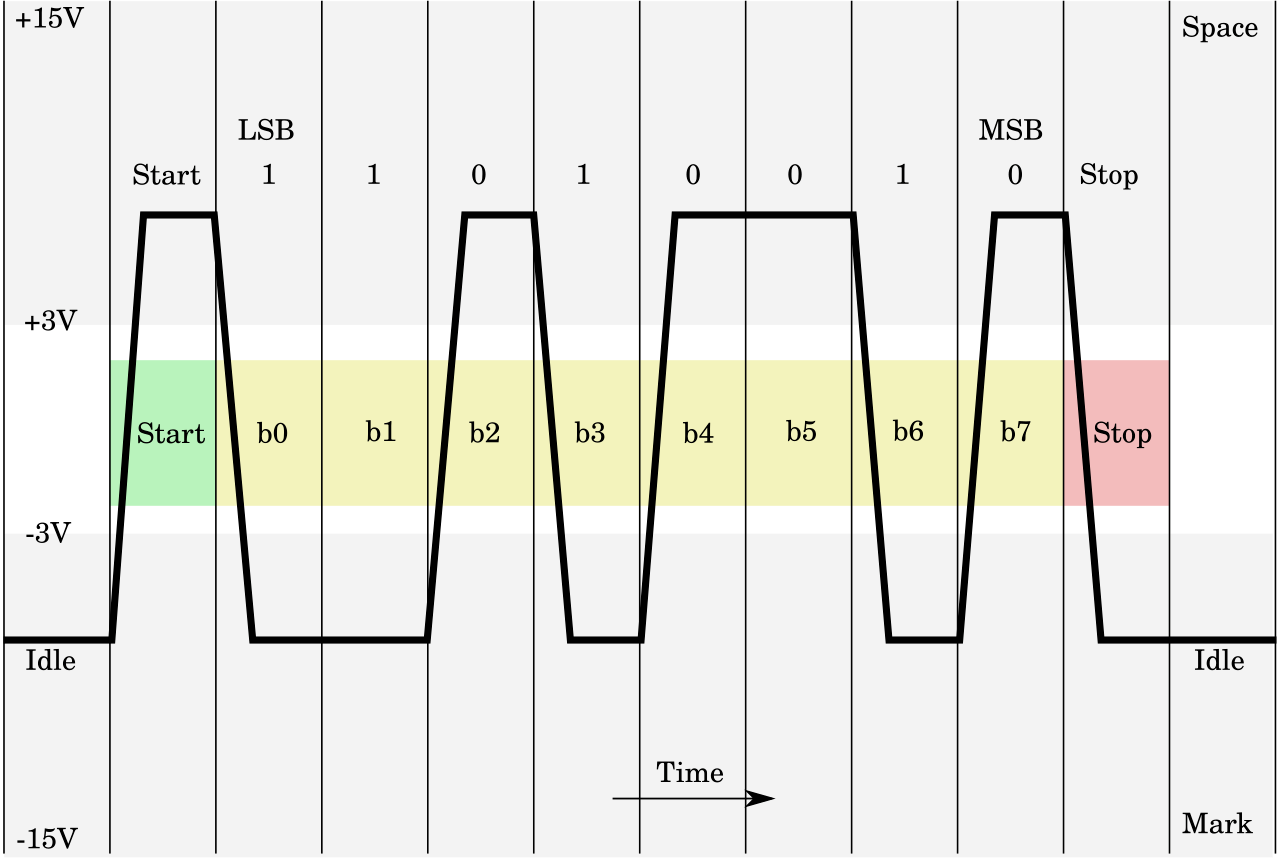
\includegraphics[width=0.8\textwidth, height=0.20\textheight, keepaspectratio]{figure/RS232-parameters.png}
                \caption[Illustration of RS232 parameters]{By $Rs232_oscilloscope_trace.jpg$: Ktnbnderivative work: Samuel Tardieu (talk)  $Rs232_oscilloscope_trace.jpg$, CC SA 1.0, \hyperlink{https://commons.wikimedia.org/w/index.php?curid=6101703}{https://commons.wikimedia.org/w/index.php?curid=6101703}  \autocite{RS2322026}}\label{fig:RS232}
            \end{figure}

            \cleardoublepage

        \section{(cV) Using QEI to detect the direction of rotation}\label{sec:cV}

            Quadrature Encoder Interface (QEI) is a method used to determine the position and direction of rotation of a motor shaft. It uses two signals, typically referred to as A and B, which are generated by the encoder as the shaft rotates. \autocite{Section15Quadrature}
            The Quadrature Encoder Interface (QEI) provides an interface to incremental encoders for obtaining mechanical position and speed data from rotating systems, enabling closed-loop motor control. A typical quadrature encoder consists of a slotted wheel mounted on the motor shaft and an emitter/detector module that senses the slots, producing two phase-shifted output signals, see figure \ref{fig:QEI}, Phase A (QEAx) and Phase B (QEBx), along with an Index pulse (INDXx) that marks a reference position once per mechanical revolution. The relative phase between QEAx and QEBx encodes the direction of rotation, while a 16-bit Up/Down Counter (POSxCNT) tracks the angular position by incrementing or decrementing on each state transition. \autocite{Section15Quadrature}

            \begin{figure}
                \centering
                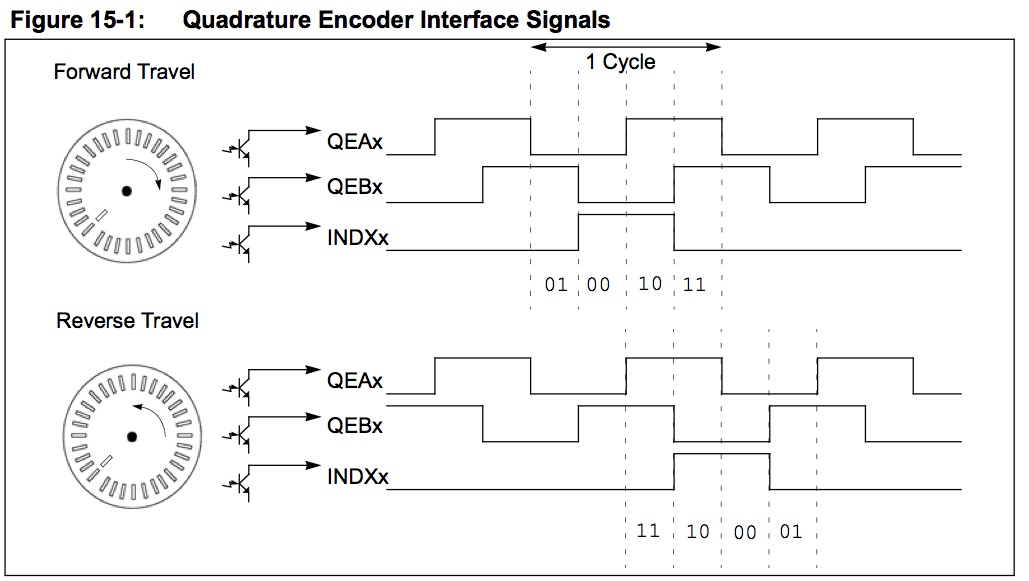
\includegraphics[width=0.8\textwidth, height=0.20\textheight, keepaspectratio]{figure/QEI.png}
                \caption{Illustration of Quadrature Encoder Interface (QEI) signals\autocite{Section15Quadrature}}
                \label{fig:QEI}
            \end{figure}

            To illustrate the operating principle, consider a slotted disk mounted on the motor shaft with $N = 360$ evenly spaced slots around its circumference, sensed by two laser-based optical detectors offset by a quarter slot pitch (i.e.\ \SI{90}{\degree} electrical phase shift). As the disk rotates, each detector produces a square wave: detector A generates QEAx and detector B generates QEBx, with both signals running at the same frequency but offset in phase. For forward rotation, QEAx leads QEBx by \SI{90}{\degree}, so the (QEAx,~QEBx) pair cycles through the state sequence $00 \rightarrow 10 \rightarrow 11 \rightarrow 01 \rightarrow 00$; for reverse rotation, the sequence is traversed in the opposite order. Each transition between states is counted, yielding $4N = 1440$ counts per mechanical revolution and an angular resolution of \SI{0.25}{\degree}. At a shaft speed of, for example, \SI{600}{rpm} (\SI{10}{\hertz}), the QEAx and QEBx signals oscillate at \SI{3.6}{\kilo\hertz} and the counter POSxCNT updates at \SI{14.4}{\kilo\hertz}, incrementing for forward rotation and decrementing for reverse. Once per revolution, the INDXx pulse asserts and can be used to reset POSxCNT, providing an absolute reference that eliminates accumulated drift.

            To visuallize and confirm the direction of rotation, the experiment described in Section \ref{ch:ExperimentT3} has been performed, where the QEI signals were recorded while the motor was driven in both forward and reverse directions. The resulting QEI identifies the direction of rotation.
            
            \begin{figure}[ht]
                \centering
                \begin{minipage}[c]{0.60\textwidth}
                    \centering
                    \vspace{0pt}
                    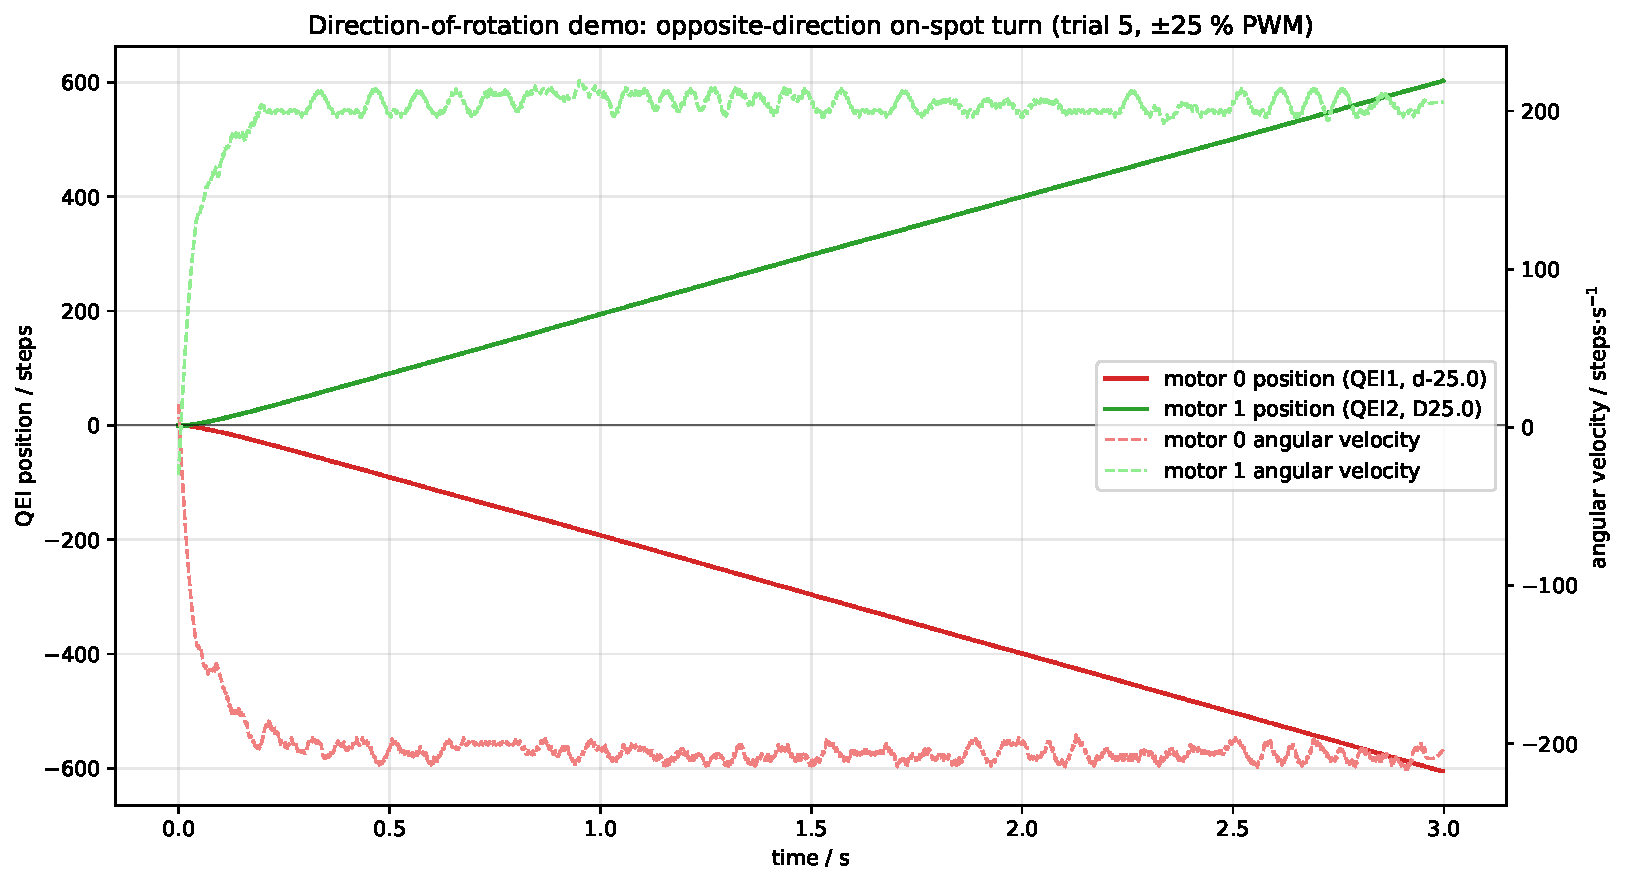
\includegraphics[width=\linewidth]{figure/qei-direction-of-rotation.pdf}
                \end{minipage}\hfill
                \begin{minipage}[c]{0.36\textwidth}
                    \centering
                    \vspace{0pt}
                    \href{https://youtu.be/qWWmoOZy7aw}{%
                        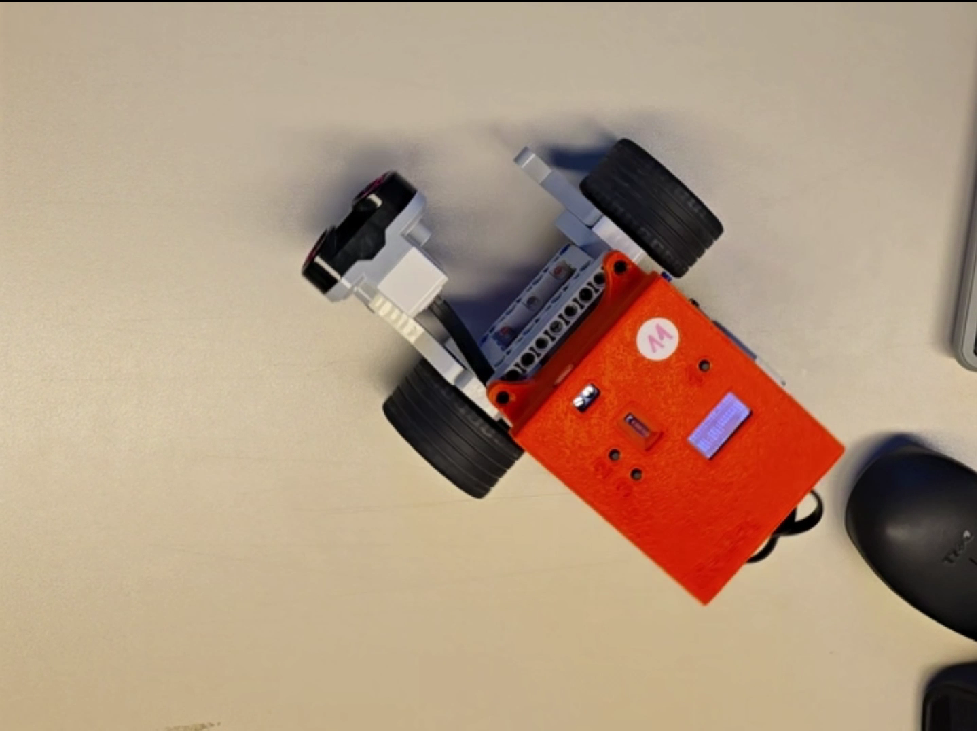
\includegraphics[width=\linewidth]{figure/vid/Screenshot 2026-05-02 015815.png}%
                    }%
                    \\[-2pt]
                    {\footnotesize \href{https://youtu.be/qWWmoOZy7aw}{\url{https://youtu.be/qWWmoOZy7aw}}}
                \end{minipage}
                \caption[Opposite-direction on-spot turn at $\pm$25\,\% PWM]{Opposite-direction on-spot turn at $\pm$25\,\% PWM. Left: motor~0 (red, \texttt{d-25.0}) and motor~1 (green, \texttt{D25.0}); solid lines show QEI position (left axis), dashed lines show angular velocity (right axis). Right: inline video of the on-spot turn.}
                \label{fig:qei-direction}
            \end{figure}

            \cleardoublepage
        
        \section{(dV) Review of documentation for Serial.ICE}
            From the documentation of Serial.ICE the following key information can be extracted:
            \begin{itemize}
                \item 2 options to send data I: through the direk-in main field and II: through the `Data to send' field. 
                \item Data is received in the `Main window' field and shown here.
                \item Logging: in the `Serial window' click on `LogtoFile' to log the communication to a file. The file is saved in the same directory as Serial.ICE.exe.
            \end{itemize}

            The necessary commands are $D25.0$, $D50.0$, $D75.0$, and $D100.0$ to set the duty cycle of the PWM signal to \SI{25}{\percent}, \SI{50}{\percent}, \SI{75}{\percent}, and \SI{100}{\percent} respectively.

            Based on this objective, a standardized test plan is implemented: (i) Define communication parameters (3.0 Mbaud, 8N1, no parity/flow control), (ii) Set the drive to PWM constant mode, (iii) reset the QEI counter and document environmental conditions, (iv) for each speed level, perform a jump from a standstill and fully log the response. This provides reproducible data sets that can subsequently be evaluated in a comparable manner.

            \cleardoublepage




    \chapter{Experiment T3: RetBot system identification, part I}\label{ch:ExperimentT3}
        The EV3 robot was controlled via Serial.ICE using USB/virtual COM port. In constant PWM mode, symmetrical duty cycles of \SI{25}{\percent}, \SI{50}{\percent}, \SI{75}{\percent}, and \SI{100}{\percent} were initially set for both drives (d/D refer to motors 0/1). To ensure complete traceability, the following standardized procedure was followed:

        \begin{itemize}
            \item 1. Connect and configure: Plug in the EV3 via USB, open Serial.ICE, set communication parameters (e.g., 3.0 MBaud, 8N1, no parity/flow control), optionally send v (version) and r (QEI reset).
            \item 2. Set PWM and start logging: Select mode (m1), command desired PWM (d /D, e.g., d50.0, D50.0). Activate the log function in Serial.ICE so that commands and responses are recorded.
            \item 3. Positioning and test run: Disconnect the USB cable, position the robot as defined on the track. Start the test locally on the device by pressing button 2; press button 2 again to stop. (The controller block centrally controls the inputs and outputs.)
            \item 4. Retrieve and save measurement data: Reconnect the robot, send the command g in Serial.ICE to read the measurement data from the controller. Save/close the log file using the Log button.
            \item 5. Repeat for all duty cycles: Repeat steps \numrange{1}{4} for \SI{25}{\percent}, \SI{50}{\percent}, \SI{75}{\percent}, \SI{100}{\percent}, and, if applicable, for asymmetric settings (e.g., d25/D24, d50/D47, d75/D71, d100/D95) to improve tracking and compensate for motor differences.
        \end{itemize}

    
        \section{(e) Documentation of communication with the RetBot}
            
            \todo[inline]{add description of commands used and the output}
            communication
            r - reset QEI counter
            - output: NA
            d25.0 - set duty cycle of motor 0 to 25%
            D25.0 - set duty cycle of motor 1 to 25%
            - output: NA
            g - get data 
            - output: all recorded data -> then saved to file
            - exerpt of log file:
            \todo[inline]{format the data in the log file and put it here using listing}
            {\tiny
            \begin{verbatim}
                fsample=500Hz
                Time/ms;QEI1/steps;QEI2/steps;d/cm;Mot0/%
                0;   0;   0; 32.0;  0
                2;   0;   0; 32.0;  0
                4;   0;   0; 32.0;  0
                6;   0;   0; 32.0;  0
                8;   0;   0; 32.0;  0
                10;   0;   0; 32.0;  0
                12;   0;   0; 32.0;  0
                14;   0;   0; 32.0;  0
                16;   0;   0; 32.0;  0
                18;   0;   0; 32.0;  0
                20;   0;   0; 32.0;  0
                22;   0;   0; 32.0;  0
                24;   0;   0; 32.0;  0
                26;   0;   1; 32.0;  0
                28;   0;   1; 32.0;  0
                30;   0;   1; 32.0;  0
                32;   0;   1; 32.0;  0
                34;   0;   2; 32.0;  0
                36;   0;   2; 32.0;  0
                38;   0;   2; 32.0;  0
                40;   0;   2; 32.0; 25
                42;   0;   3; 32.0; 25
                44;   0;   3; 32.0; 25
                46;   0;   3; 32.0; 25
                48;   0;   4; 32.0; 25
                50;   0;   4; 32.0; 25
                52;   0;   4; 32.0; 25
                54;   0;   4; 32.0; 25
                56;   0;   5; 32.0; 25
                58;   1;   5; 32.0; 25
                60;   1;   6; 32.0; 25
                62;   1;   6; 32.0; 25
                64;   1;   6; 32.0; 25
                66;   1;   6; 32.0; 25
                68;   2;   7; 32.0; 25
                70;   2;   7; 32.0; 25
                72;   2;   8; 32.0; 25
                74;   2;   8; 32.0; 25
                76;   2;   8; 32.0; 25
                78;   3;   9; 32.0; 25
                80;   3;   9; 32.0; 25
                82;   3;   9; 32.0; 25
                84;   4;  10; 32.0; 25
                86;   4;  10; 32.0; 25
                88;   4;  10; 32.0; 25
                90;   4;  11; 32.0; 25
                92;   5;  11; 32.0; 25
                94;   5;  12; 32.0; 25
                96;   5;  12; 32.0; 25
                98;   6;  12; 32.0; 25
                100;   6;  13; 32.0; 25
            \end{verbatim}
            }

            \todo[inline]{add a description of the observed behavior, e.g., the left deviation/drivt of the robot, the time it takes to reach a steady state, the maximum velocity reached, and any other interesting observations.}

            \todo[inline]{add a description of the offset behavior in the 25\% duty cycle, the derivative of the velocity, showing the spike at the point}


        \section{(f) Analysis of the RetBot's drive train}
            The goal of the analysis is to quantitatively describe the drive dynamics based on the recorded QEI signals (positions) and the velocities derived from them.
            The QEI time series were preprocessed for each duty cycle (uniform time base, offset correction), and the velocity was determined as a smoothed time derivative; this reduces high-frequency quantization and differentiation noise without significantly distorting the transient response.

            \todo[inline]{add description of the smoothing method used, e.g., Savitzky--Golay filter with specific parameters}

            \missingfigure{TASK: import the data into Matlab and draw one graph per drive train containing the four different conditions and}


            
            \subsection{Interpretation}\label{sec:Interpretation}
            \todo[inline]{add short interpretation paragraph}

            \subsection{Conclusion}\label{sec:Conclusion}
            \todo[inline]{add short conclusion paragraph}
            





    \appendix
        % \makeatletter
        
    \chapter{Appendix Frontmatter}

        \section{Declarations}\label{app:statutory}

            \begin{enumerate}
                \item Wir erkläre hiermit, dass wir dieses Dokument selbstständig verfasst, noch nicht anderweitig für Prüfungszwecke vorgelegt, keine anderen als die angegebenen Quellen und Hilfsmittel benutzt sowie wörtliche und sinngemäße Zitate als solche gekennzeichnet haben.
            \end{enumerate}

            \vskip22mm
            Regensburg, den 2026-05-01, \\
            -\hskip6cm Marius Off\hskip2cm $Matrikelnummer:3416002$,\\
            "\hskip6cm Janis Graf\hskip2cm $Matrikelnummer:3377251$
            \vskip1mm
            \hrule
            \vskip1mm
            {\footnotesize Ort, Datum und Unterschrift}

            \vspace{12mm}

            \cleardoublepage

        \listoffigures

        \listoftables

            \cleardoublepage

    \chapter{Appendix Code and Resources}

            \section{Video resources}

            \begin{figure}[ht]
                \centering
                \begin{minipage}[c]{0.48\textwidth}
                    \centering
                    \vspace{0pt}
                    \href{https://youtu.be/q9igvjXbKiY}{%
                        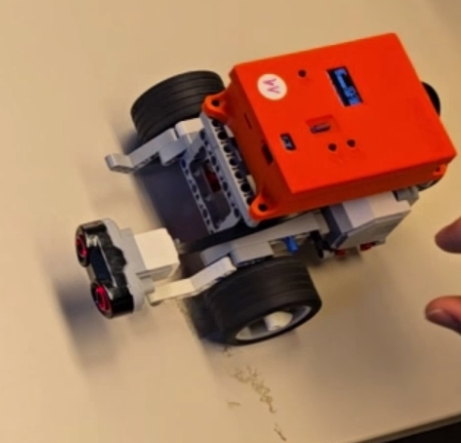
\includegraphics[width=\linewidth]{figure/vid/image-25per.png}%
                    }%
                    \\[-2pt]
                    {\footnotesize 25\% duty cycle}\\[-2pt]
                    {\footnotesize \href{https://youtu.be/q9igvjXbKiY}{\url{https://youtu.be/q9igvjXbKiY}}}
                \end{minipage}\hfill
                \begin{minipage}[c]{0.48\textwidth}
                    \centering
                    \vspace{0pt}
                    \href{https://youtu.be/n6qsIMwFsFM}{%
                        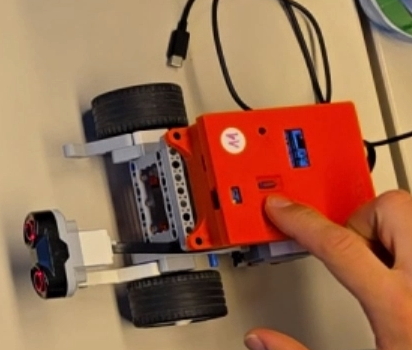
\includegraphics[width=\linewidth]{figure/vid/image-75per.png}%
                    }%
                    \\[-2pt]
                    {\footnotesize 75\% duty cycle}\\[-2pt]
                    {\footnotesize \href{https://youtu.be/n6qsIMwFsFM}{\url{https://youtu.be/n6qsIMwFsFM}}}
                \end{minipage}
                \caption{Videos of the RetBot moving alongside a folding rule at two duty cycles.}
                \label{fig:duty-cycle-videos}
            \end{figure}

            \section{Code used for the analysis of the Preperations}

            %\lstinputlisting[caption={Code used for the analysis of the Preperations}, label={lst:preperations}]{../02_Preperations/RTP-T2-analysis.ipynb}
        
    \chapter{Appendix extra calculations}
        NOTE: This chapter exists because I cant read instructions and somehow thought that it would be interesting to calculate the movement and rotation of the robot based on the QEI data.

        \section{Differential-drive kinematics from QEI}\label{sec:diffdrive}

            Under the standard \emph{differential-drive / no-slip} assumption the body-frame trajectory of the RetBot can be reconstructed from the two QEI counters alone. The convention used here is \texttt{QEI1} = motor~0 = left wheel, \texttt{QEI2} = motor~1 = right wheel; the wheel radius is~$r$, the wheel separation~$L$, and \(\mathrm{CPR}\) the encoder counts per wheel revolution (after the gearbox). The encoder counts are first mapped to wheel angles and per-wheel arc lengths,

            \begin{equation}
                \theta_{L,R}(t) = \frac{\mathrm{steps}_{L,R}(t)}{\mathrm{CPR}}\,2\pi,
                \qquad
                s_{L,R}(t) = r\,\theta_{L,R}(t).
                \label{eq:diffdrive-wheel}
            \end{equation}

            The body-frame forward path length and cumulative heading then follow as the average and length-normalised difference of the wheel arcs,

            \begin{equation}
                s(t) = \tfrac{1}{2}\!\left(s_R(t) + s_L(t)\right),
                \qquad
                \varphi(t) = \frac{s_R(t) - s_L(t)}{L},
                \label{eq:diffdrive-body}
            \end{equation}

            with $\varphi > 0$ counterclockwise viewed from above. The body-frame velocities are obtained as smoothed time derivatives, $v = \dot s$ and $\omega = \dot\varphi$, using the same Savitzky--Golay filter described in Section~\ref{sec:Interpretation}. The resulting forward distance and heading change for the four main duty cycles are shown in Figure~\ref{fig:diffdrive-distance-heading}.

            \begin{figure}[ht]
                \centering
                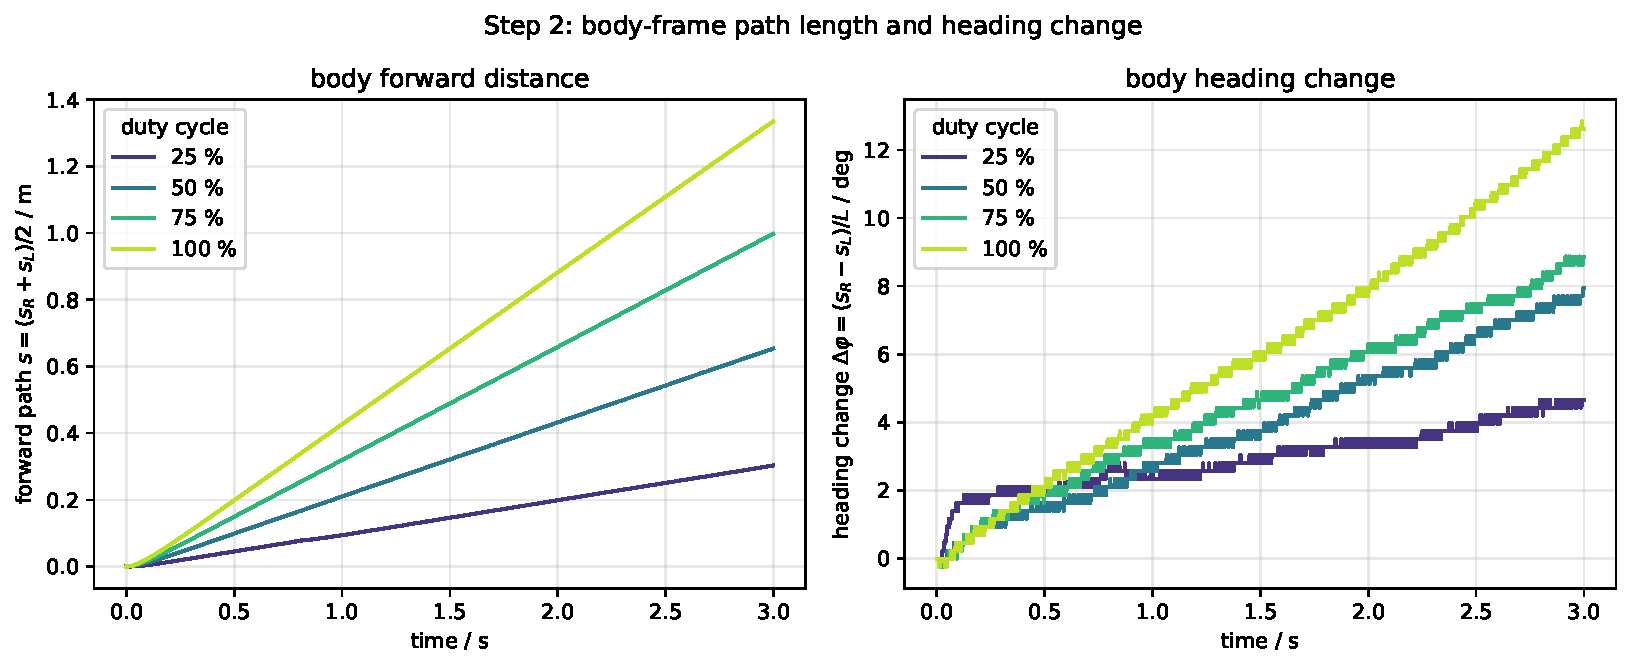
\includegraphics[width=\textwidth]{figure/differential-drive-distance-heading.pdf}
                \caption[Body-frame forward path $s$ (left) and cumulative heading change $\Delta\varphi$ (right)]{Body-frame forward path $s$ (left) and cumulative heading change $\Delta\varphi$ (right) from~\eqref{eq:diffdrive-body} for the four main duty cycles. The non-zero heading is the integrated effect of the right wheel consistently leading the left.}
                \label{fig:diffdrive-distance-heading}
            \end{figure}
            
            The world-frame pose $(x, y, \varphi)$ is obtained by discrete integration of the body-frame quantities. Treating each sample interval as a short circular arc of length $\Delta s_k$ and turn angle $\Delta\varphi_k$, the midpoint-heading update is second-order accurate under non-zero curvature:

            \begin{align}
                \varphi_k &= \varphi_{k-1} + \Delta\varphi_k,
                \label{eq:diffdrive-pose-phi} \\
                x_k &= x_{k-1} + \Delta s_k \cos\!\left(\varphi_{k-1} + \tfrac{1}{2}\Delta\varphi_k\right),
                \label{eq:diffdrive-pose-x} \\
                y_k &= y_{k-1} + \Delta s_k \sin\!\left(\varphi_{k-1} + \tfrac{1}{2}\Delta\varphi_k\right),
                \label{eq:diffdrive-pose-y}
            \end{align}

            starting from $(x_0, y_0, \varphi_0) = (0, 0, 0)$. The reconstructed trajectories for the four constant-PWM drives plus the opposite-direction on-spot turn at $\pm 25\,\%$ are shown in Figure~\ref{fig:differential-drive-trajectory}.

            \begin{figure}[ht]
                \centering
                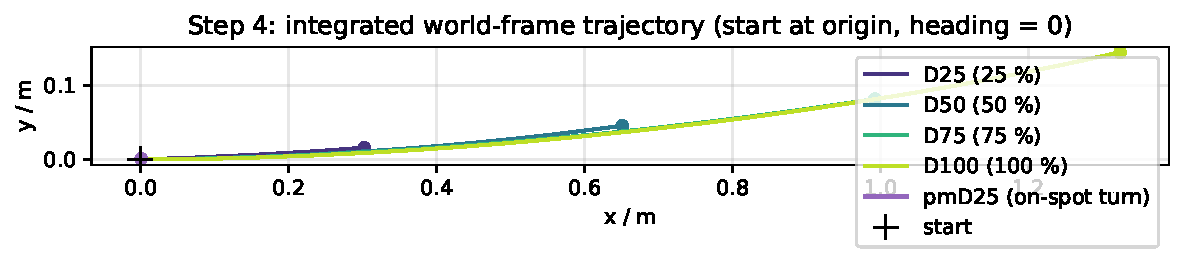
\includegraphics[width=0.7\textwidth]{figure/differential-drive-trajectory.pdf}
                \caption[Reconstructed world-frame trajectories]{Reconstructed world-frame trajectories under~\eqref{eq:diffdrive-pose-phi}--\eqref{eq:diffdrive-pose-y} ($r = 28$\,mm, $L = 120$\,mm, $\mathrm{CPR} = 360$). Straight drives at \SIrange{25}{100}{\percent} PWM curve slightly leftward (right wheel leads); the $\pm 25\,\%$ on-spot turn produces $\approx 282^{\circ}$ of net rotation with $s \approx 0$.}
                \label{fig:differential-drive-trajectory}
            \end{figure}

            The on-spot turn provides a clean self-consistency check for the kinematics: with wheel commands of opposite sign and equal magnitude the arcs satisfy $s_L \approx -s_R$, so by~\eqref{eq:diffdrive-body} the body-frame forward path collapses to $s \approx 0$ while $\varphi$ accumulates linearly --- exactly as observed (final $s = -0.1\,\mathrm{mm}$, $\Delta\varphi = +281.9^{\circ}$ over the $\SI{3}{\second}$ log). The robot parameters used here are estimates for an EV3 educational chassis; an absolute calibration of $r$ against a measured reference distance would scale~$s$ correctly, while heading accuracy in turns is governed only by the ratio $r/L$.

        \section{Calculation of the derivatives and integrals of the motor position}
            \todo[inline]{add description of the method used to calculate the derivatives and integrals, e.g., numerical differentiation and integration techniques, and any smoothing applied to the data. add it from the notebook.}

            \missingfigure{add figure d50-integral-derivative-chain.pdf to the text above}\label{fig:d50-integral-derivative-chain}

        %%%%%%%%%%%%%%%%%%%%%%%%%%%%%%%%%%%%%%%%%%%%%%%%%%%%%%%%%%%%%%%%%%%%%
        %\chapter{Bibliography}
        %%%Literaturverzeichnis
        \printbibliography

        %%%%%%%%%%%%%%%%%%%%%%%%%%%%%%%%%%%%%%%%%%%%%%%%%%%%%%%%%%%%%%%%%%%%%

\end{document}